\chapter{Algoritmos voraces}

\index{algoritmo voraz}

Un \key{algoritmo voraz}
construye una solución al problema
tomando siempre la decisión que parece
mejor en ese momento.
Un algoritmo voraz nunca revoca
sus decisiones, sino que construye directamente
la solución final.
Por esta razón, los algoritmos voraces
suelen ser muy eficientes.

La dificultad en el diseño de algoritmos voraces
es encontrar una estrategia voraz
que siempre produzca una solución óptima
al problema.
Las decisiones localmente óptimas en un algoritmo voraz
también deberían ser globalmente óptimas.
A menudo es difícil argumentar que
un algoritmo voraz funciona.

\section{Problema de la moneda}

Como primer ejemplo, consideramos un problema
en el que se nos da un conjunto de monedas
y nuestra tarea es formar una suma de dinero $n$
usando las monedas.
Los valores de las monedas son
$\texttt{coins}=\{c_1,c_2,\ldots,c_k\}$,
y cada moneda se puede usar tantas veces como queramos.
¿Cuál es el número mínimo de monedas necesarias?

Por ejemplo, si las monedas son las monedas de euro (en céntimos)
\[\{1,2,5,10,20,50,100,200\}\]
y $n=520$,
necesitamos al menos cuatro monedas.
La solución óptima es seleccionar monedas
$200+200+100+20$ cuya suma es 520.

\subsubsection{Algoritmo voraz}

Un algoritmo voraz simple para el problema
siempre selecciona la moneda más grande posible,
hasta que se ha construido la suma de dinero requerida.
Este algoritmo funciona en el caso de ejemplo,
porque primero seleccionamos dos monedas de 200 céntimos,
luego una moneda de 100 céntimos y finalmente una moneda de 20 céntimos.
¿Pero este algoritmo siempre funciona?

Resulta que si las monedas son las monedas de euro,
el algoritmo voraz \emph{siempre} funciona, es decir,
siempre produce una solución con el menor
número posible de monedas.
La corrección del algoritmo se puede
mostrar como sigue:

Primero, cada moneda 1, 5, 10, 50 y 100 aparece
como máximo una vez en una solución óptima,
porque si la
solución contendría dos de esas monedas,
podríamos reemplazarlas por una moneda y
obtener una mejor solución.
Por ejemplo, si la solución contendría
monedas $5+5$, podríamos reemplazarlas por la moneda $10$.

De la misma manera, las monedas 2 y 20 aparecen
como máximo dos veces en una solución óptima,
porque podríamos reemplazar
monedas $2+2+2$ por monedas $5+1$ y
monedas $20+20+20$ por monedas $50+10$.
Además, una solución óptima no puede contener
monedas $2+2+1$ o $20+20+10$,
porque podríamos reemplazarlas por monedas $5$ y $50$.

Usando estas observaciones,
podemos mostrar para cada moneda $x$ que
no es posible construir óptimamente
una suma $x$ o cualquier suma mayor usando solo monedas
que son más pequeñas que $x$.
Por ejemplo, si $x=100$, la suma óptima más grande
usando las monedas más pequeñas es  $50+20+20+5+2+2=99$.
Por lo tanto, el algoritmo voraz que siempre selecciona
la moneda más grande produce la solución óptima.

Este ejemplo muestra que puede ser difícil
argumentar que un algoritmo voraz funciona,
incluso si el algoritmo en sí es simple.

\subsubsection{Caso general}

En el caso general, el conjunto de monedas puede contener cualquier moneda
y el algoritmo voraz \emph{no} produce necesariamente
una solución óptima.

Podemos probar que un algoritmo voraz no funciona
mostrando un contraejemplo
donde el algoritmo da una respuesta incorrecta.
En este problema podemos encontrar fácilmente un contraejemplo:
si las monedas son $\{1,3,4\}$ y la suma objetivo
es 6, el algoritmo voraz produce la solución
$4+1+1$ mientras que la solución óptima es $3+3$.

No se sabe si el problema general de la moneda
se puede resolver usando algún algoritmo voraz\footnote{Sin embargo, es posible
\emph{comprobar} en tiempo polinomial
si el algoritmo voraz presentado en este capítulo funciona para
un conjunto dado de monedas \cite{pea05}.}.
Sin embargo, como veremos en el Capítulo 7,
en algunos casos,
el problema general se puede resolver de manera eficiente
utilizando un algoritmo de programación dinámica que siempre da la
respuesta correcta.

\section{Planificación}

Muchos problemas de planificación se pueden resolver
usando algoritmos voraces.
Un problema clásico es el siguiente:
Dado $n$ eventos con sus tiempos de inicio y fin,
encuentra un horario
que incluya tantos eventos como sea posible.
No es posible seleccionar un evento parcialmente.
Por ejemplo, considere los siguientes eventos:
\begin{center}
\begin{tabular}{lll}
evento & tiempo de inicio & tiempo de fin \\
\hline
$A$ & 1 & 3 \\
$B$ & 2 & 5 \\
$C$ & 3 & 9 \\
$D$ & 6 & 8 \\
\end{tabular}
\end{center}
En este caso, el número máximo de eventos es dos.
Por ejemplo, podemos seleccionar los eventos $B$ y $D$
de la siguiente manera:
\begin{center}
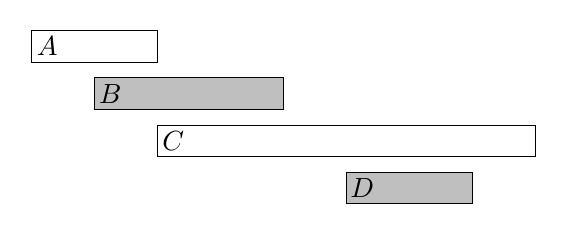
\begin{tikzpicture}[scale=.4]
  \begin{scope}
    \draw (2, 0) rectangle (6, -1);
    \draw[fill=lightgray] (4, -1.5) rectangle (10, -2.5);
    \draw (6, -3) rectangle (18, -4);
    \draw[fill=lightgray] (12, -4.5) rectangle (16, -5.5);
    \node at (2.5,-0.5) {$A$};
    \node at (4.5,-2) {$B$};
    \node at (6.5,-3.5) {$C$};
    \node at (12.5,-5) {$D$};
  \end{scope}
\end{tikzpicture}
\end{center}

Es posible inventar varios algoritmos voraces
para el problema, pero ¿cuál de ellos funciona en todos los casos?

\subsubsection*{Algoritmo 1}
La primera idea es seleccionar eventos tan \emph{cortos} como sea posible.
En el caso del ejemplo, este algoritmo
selecciona los siguientes eventos:
\begin{center}
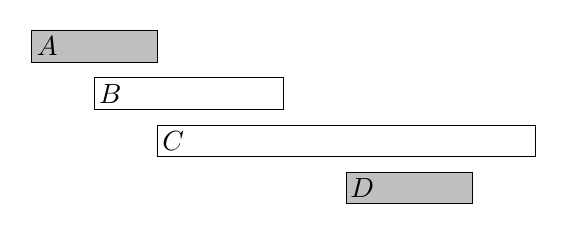
\begin{tikzpicture}[scale=.4]
  \begin{scope}
    \draw[fill=lightgray] (2, 0) rectangle (6, -1);
    \draw (4, -1.5) rectangle (10, -2.5);
    \draw (6, -3) rectangle (18, -4);
    \draw[fill=lightgray] (12, -4.5) rectangle (16, -5.5);
    \node at (2.5,-0.5) {$A$};
    \node at (4.5,-2) {$B$};
    \node at (6.5,-3.5) {$C$};
    \node at (12.5,-5) {$D$};
  \end{scope}
\end{tikzpicture}
\end{center}

Sin embargo, seleccionar eventos cortos no siempre
es una estrategia correcta. Por ejemplo, el algoritmo falla
en el siguiente caso:
\begin{center}
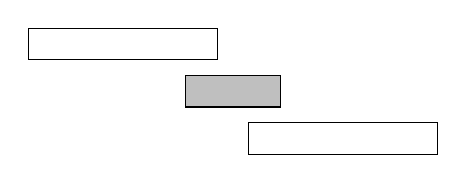
\begin{tikzpicture}[scale=.4]
  \begin{scope}
    \draw (1, 0) rectangle (7, -1);
    \draw[fill=lightgray] (6, -1.5) rectangle (9, -2.5);
    \draw (8, -3) rectangle (14, -4);
  \end{scope}
\end{tikzpicture}
\end{center}
Si seleccionamos el evento corto, solo podemos seleccionar un evento.
Sin embargo, sería posible seleccionar ambos eventos largos.

\subsubsection*{Algoritmo 2}

Otra idea es siempre seleccionar el siguiente posible
evento que \emph{comience} lo más \emph{temprano} posible.
Este algoritmo selecciona los siguientes eventos:
\begin{center}
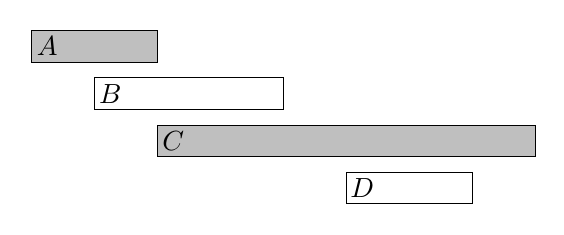
\begin{tikzpicture}[scale=.4]
  \begin{scope}
    \draw[fill=lightgray] (2, 0) rectangle (6, -1);
    \draw (4, -1.5) rectangle (10, -2.5);
    \draw[fill=lightgray] (6, -3) rectangle (18, -4);
    \draw (12, -4.5) rectangle (16, -5.5);
    \node at (2.5,-0.5) {$A$};
    \node at (4.5,-2) {$B$};
    \node at (6.5,-3.5) {$C$};
    \node at (12.5,-5) {$D$};
  \end{scope}
\end{tikzpicture}
\end{center}

Sin embargo, podemos encontrar un contraejemplo
también para este algoritmo.
Por ejemplo, en el siguiente caso,
el algoritmo solo selecciona un evento:
\begin{center}
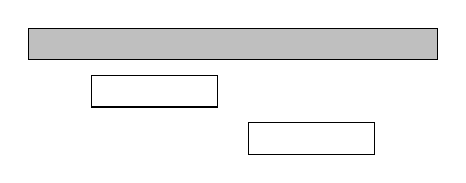
\begin{tikzpicture}[scale=.4]
  \begin{scope}
    \draw[fill=lightgray] (1, 0) rectangle (14, -1);
    \draw (3, -1.5) rectangle (7, -2.5);
    \draw (8, -3) rectangle (12, -4);
  \end{scope}
\end{tikzpicture}
\end{center}
Si seleccionamos el primer evento, no es posible
seleccionar ningún otro evento.
Sin embargo, sería posible seleccionar los
otros dos eventos.

\subsubsection*{Algoritmo 3}

La tercera idea es siempre seleccionar el siguiente
evento posible que \emph{termine} lo más \emph{temprano} posible.
Este algoritmo selecciona los siguientes eventos: 
\begin{center}
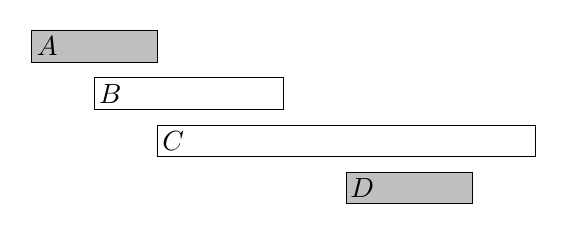
\begin{tikzpicture}[scale=.4]
  \begin{scope}
    \draw[fill=lightgray] (2, 0) rectangle (6, -1);
    \draw (4, -1.5) rectangle (10, -2.5);
    \draw (6, -3) rectangle (18, -4);
    \draw[fill=lightgray] (12, -4.5) rectangle (16, -5.5);
    \node at (2.5,-0.5) {$A$};
    \node at (4.5,-2) {$B$};
    \node at (6.5,-3.5) {$C$};
    \node at (12.5,-5) {$D$};
  \end{scope}
\end{tikzpicture}
\end{center}

Resulta que este algoritmo
\emph{siempre} produce una solución óptima.
La razón de esto es que siempre es una opción óptima
seleccionar primero un evento que termine
lo más temprano posible.
Después de esto, es una opción óptima
seleccionar el siguiente evento
usando la misma estrategia, etc.,
hasta que no podamos seleccionar más eventos.

Una forma de argumentar que el algoritmo funciona
es considerar
qué sucede si primero seleccionamos un evento
que termina más tarde que el evento que termina
lo más temprano posible.
Ahora, tendremos como máximo un número igual de
opciones sobre cómo podemos seleccionar el siguiente evento.
Por lo tanto, seleccionar un evento que termina más tarde
nunca puede producir una mejor solución,
y el algoritmo voraz es correcto.

\section{Tareas y plazos}

Consideremos ahora un problema donde
se nos dan $n$ tareas con duraciones y plazos
y nuestra tarea es elegir un orden para realizar las tareas.
Para cada tarea, ganamos $d-x$ puntos
donde $d$ es el plazo de la tarea
y $x$ es el momento en que terminamos la tarea.
¿Cuál es la mayor puntuación total posible
que podemos obtener?

Por ejemplo, supongamos que las tareas son las siguientes:
\begin{center}
\begin{tabular}{lll}
tarea & duración & plazo \\
\hline
$A$ & 4 & 2 \\
$B$ & 3 & 5 \\
$C$ & 2 & 7 \\
$D$ & 4 & 5 \\
\end{tabular}
\end{center}
En este caso, un programa óptimo para las tareas
es el siguiente:
\begin{center}
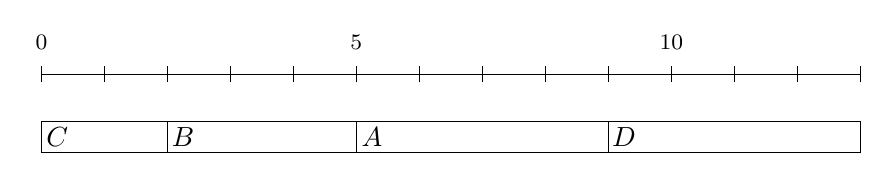
\begin{tikzpicture}[scale=.4]
  \begin{scope}
    \draw (0, 0) rectangle (4, -1);
    \draw (4, 0) rectangle (10, -1);
    \draw (10, 0) rectangle (18, -1);
    \draw (18, 0) rectangle (26, -1);
    \node at (0.5,-0.5) {$C$};
    \node at (4.5,-0.5) {$B$};
    \node at (10.5,-0.5) {$A$};
    \node at (18.5,-0.5) {$D$};

    \draw (0,1.5) -- (26,1.5);
    \foreach \i in {0,2,...,26}
    {
        \draw (\i,1.25) -- (\i,1.75);
    }
    \footnotesize
    \node at (0,2.5) {0};
    \node at (10,2.5) {5};
    \node at (20,2.5) {10};

  \end{scope}
\end{tikzpicture}
\end{center}
En esta solución, $C$ produce 5 puntos,
$B$ produce 0 puntos, $A$ produce $-7$ puntos
y $D$ produce $-8$ puntos,
por lo que la puntuación total es $-10$.
Sorprendentemente, la solución óptima al problema
no depende en absoluto de las fechas límite,
sino que una estrategia codiciosa correcta es simplemente
realizar las tareas \emph{ordenadas por sus duraciones}
en orden creciente.
La razón de esto es que si alguna vez realizamos
dos tareas una después de la otra de modo que la primera tarea
dure más que la segunda tarea,
podemos obtener una mejor solución si intercambiamos las tareas.
Por ejemplo, considere el siguiente horario:
\begin{center}
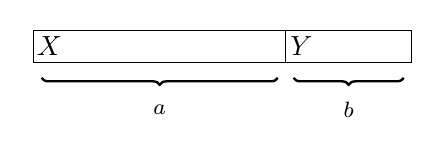
\begin{tikzpicture}[scale=.4]
  \begin{scope}
    \draw (0, 0) rectangle (8, -1);
    \draw (8, 0) rectangle (12, -1);
    \node at (0.5,-0.5) {$X$};
    \node at (8.5,-0.5) {$Y$};

\draw [decoration={brace}, decorate, line width=0.3mm] (7.75,-1.5) -- (0.25,-1.5);
\draw [decoration={brace}, decorate, line width=0.3mm] (11.75,-1.5) -- (8.25,-1.5);

\footnotesize
\node at (4,-2.5) {$a$};
\node at (10,-2.5) {$b$};

  \end{scope}
\end{tikzpicture}
\end{center}
Aquí $a>b$, por lo que debemos intercambiar las tareas:
\begin{center}
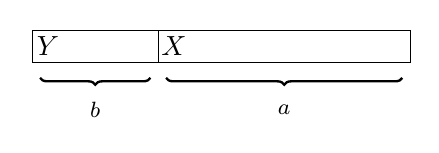
\begin{tikzpicture}[scale=.4]
  \begin{scope}
    \draw (0, 0) rectangle (4, -1);
    \draw (4, 0) rectangle (12, -1);
    \node at (0.5,-0.5) {$Y$};
    \node at (4.5,-0.5) {$X$};

\draw [decoration={brace}, decorate, line width=0.3mm] (3.75,-1.5) -- (0.25,-1.5);
\draw [decoration={brace}, decorate, line width=0.3mm] (11.75,-1.5) -- (4.25,-1.5);

\footnotesize
\node at (2,-2.5) {$b$};
\node at (8,-2.5) {$a$};

  \end{scope}
\end{tikzpicture}
\end{center}
Ahora $X$ da $b$ puntos menos e $Y$ da $a$ puntos más,
por lo que la puntuación total aumenta en $a-b > 0$.
En una solución óptima,
para dos tareas consecutivas,
debe cumplirse que la tarea más corta venga
antes de la tarea más larga.
Por lo tanto, las tareas deben realizarse
ordenadas por sus duraciones.

\section{Minimizar sumas}

A continuación, consideramos un problema en el que
se nos dan $n$ números $a_1,a_2,\ldots,a_n$
y nuestra tarea es encontrar un valor $x$
que minimice la suma
\[|a_1-x|^c+|a_2-x|^c+\cdots+|a_n-x|^c.\]
Nos centramos en los casos $c=1$ y $c=2$.

\subsubsection{Caso $c=1$}

En este caso, debemos minimizar la suma
\[|a_1-x|+|a_2-x|+\cdots+|a_n-x|.\]
Por ejemplo, si los números son $[1,2,9,2,6]$,
la mejor solución es seleccionar $x=2$
que produce la suma
\[
|1-2|+|2-2|+|9-2|+|2-2|+|6-2|=12.
\]
En el caso general, la mejor opción para $x$
es la \textit{mediana} de los números,
es decir, el número del medio después de la ordenación.
Por ejemplo, la lista $[1,2,9,2,6]$
se convierte en $[1,2,2,6,9]$ después de la ordenación,
por lo que la mediana es 2.

La mediana es una opción óptima,
porque si $x$ es menor que la mediana,
la suma se hace más pequeña al aumentar $x$,
y si $x$ es mayor que la mediana,
la suma se hace más pequeña al disminuir $x$.
Por lo tanto, la solución óptima es que $x$
sea la mediana.
Si $n$ es par y hay dos medianas,
tanto las medianas como todos los valores entre ellas
son opciones óptimas.

\subsubsection{Caso $c=2$}

En este caso, debemos minimizar la suma
\[(a_1-x)^2+(a_2-x)^2+\cdots+(a_n-x)^2.\]
Por ejemplo, si los números son $[1,2,9,2,6]$,
la mejor solución es seleccionar $x=4$
que produce la suma
\[
(1-4)^2+(2-4)^2+(9-4)^2+(2-4)^2+(6-4)^2=46.
\]
En el caso general, la mejor opción para $x$
es la \emph{media} de los números.
En el ejemplo, la media es $(1+2+9+2+6)/5=4$.
Este resultado se puede derivar presentando
la suma de la siguiente manera:
\[
nx^2 - 2x(a_1+a_2+\cdots+a_n) + (a_1^2+a_2^2+\cdots+a_n^2)
\]
La última parte no depende de $x$,
por lo que podemos ignorarla.
Las partes restantes forman una función
$nx^2-2xs$ donde $s=a_1+a_2+\cdots+a_n$.
Esta es una parábola que se abre hacia arriba
con raíces $x=0$ y $x=2s/n$,
y el valor mínimo es la media
de las raíces $x=s/n$, es decir,
la media de los números $a_1,a_2,\ldots,a_n$.

\section{Compresión de datos}

\index{compresión de datos}
\index{código binario}
\index{palabra de código}



Un \key{código binario} asigna a cada carácter
de una cadena una \key{palabra de código} que consiste en bits.
Podemos \emph{comprimir} la cadena usando el código binario
reemplazando cada carácter por la
palabra de código correspondiente.
Por ejemplo, el siguiente código binario
asigna palabras de código para los caracteres
\texttt{A}–\texttt{D}:
\begin{center}
\begin{tabular}{rr}
carácter & palabra de código \\
\hline
\texttt{A} & 00 \\
\texttt{B} & 01 \\
\texttt{C} & 10 \\
\texttt{D} & 11 \\
\end{tabular}
\end{center}
Este es un código de \key{longitud constante}
lo que significa que la longitud de cada
palabra de código es la misma.
Por ejemplo, podemos comprimir la cadena
\texttt{AABACDACA} como sigue:
\[00\,00\,01\,00\,10\,11\,00\,10\,00\]
Usando este código, la longitud de la cadena comprimida
es de 18 bits.
Sin embargo, podemos comprimir la cadena mejor
si usamos un código de \key{longitud variable}
donde las palabras de código pueden tener diferentes longitudes.
Entonces podemos dar palabras de código cortas para
los caracteres que aparecen a menudo
y palabras de código largas para los caracteres
que aparecen raramente.
Resulta que un código \key{óptimo}
para la cadena anterior es el siguiente:
\begin{center}
\begin{tabular}{rr}
carácter & palabra de código \\
\hline
\texttt{A} & 0 \\
\texttt{B} & 110 \\
\texttt{C} & 10 \\
\texttt{D} & 111 \\
\end{tabular}
\end{center}
Un código óptimo produce una cadena comprimida
que es lo más corta posible.
En este caso, la cadena comprimida usando
el código óptimo es
\[0\,0\,110\,0\,10\,111\,0\,10\,0,\]
por lo que solo se necesitan 15 bits en lugar de 18 bits.
Por lo tanto, gracias a un mejor código fue posible
ahorrar 3 bits en la cadena comprimida.

Requerimos que ninguna palabra de código
sea un prefijo de otra palabra de código.
Por ejemplo, no está permitido que un código
contenga ambas palabras de código 10
y 1011.
La razón de esto es que queremos
poder generar la cadena original
a partir de la cadena comprimida.
Si una palabra de código pudiera ser un prefijo de otra palabra de código,
esto no siempre sería posible.
Por ejemplo, el siguiente código no es \emph{válido}:
\begin{center}
\begin{tabular}{rr}
carácter & palabra de código \\
\hline
\texttt{A} & 10 \\
\texttt{B} & 11 \\
\texttt{C} & 1011 \\
\texttt{D} & 111 \\
\end{tabular}
\end{center}
Usando este código, no sería posible saber
si la cadena comprimida 1011 corresponde a
la cadena \texttt{AB} o la cadena \texttt{C}.

\index{Codificación de Huffman}

\subsubsection{Codificación de Huffman}

\key{Codificación de Huffman}\footnote{D. A. Huffman descubrió este método
al resolver una tarea de un curso universitario
y publicó el algoritmo en 1952 \cite{huf52}.} es un algoritmo voraz
que construye un código óptimo para
comprimir una cadena dada.
El algoritmo construye un árbol binario
basado en las frecuencias de los caracteres
en la cadena,
y la palabra de código de cada carácter se puede leer
siguiendo un camino desde la raíz hasta
el nodo correspondiente.
Un movimiento hacia la izquierda corresponde al bit 0,
y un movimiento hacia la derecha corresponde al bit 1.

Inicialmente, cada carácter de la cadena es
representado por un nodo cuyo peso es el
número de veces que el carácter aparece en la cadena.
Luego, en cada paso, dos nodos con pesos mínimos
se combinan creando
un nuevo nodo cuyo peso es la suma de los pesos
de los nodos originales.
El proceso continúa hasta que todos los nodos se han combinado.

A continuación, veremos cómo la codificación de Huffman crea
el código óptimo para la cadena
\texttt{AABACDACA}.
Inicialmente, hay cuatro nodos que corresponden
a los caracteres de la cadena:

\begin{center}
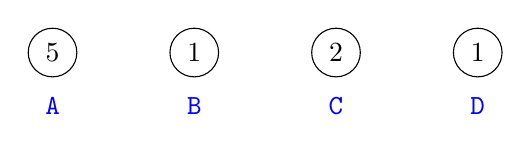
\begin{tikzpicture}[scale=0.9]
\node[draw, circle] (1) at (0,0) {$5$};
\node[draw, circle] (2) at (2,0) {$1$};
\node[draw, circle] (3) at (4,0) {$2$};
\node[draw, circle] (4) at (6,0) {$1$};

\node[color=blue] at (0,-0.75) {\texttt{A}};
\node[color=blue] at (2,-0.75) {\texttt{B}};
\node[color=blue] at (4,-0.75) {\texttt{C}};
\node[color=blue] at (6,-0.75) {\texttt{D}};

%\path[draw,thick,-] (4) -- (5);
\end{tikzpicture}
\end{center}
El nodo que representa el carácter \texttt{A}
tiene peso 5 porque el carácter \texttt{A}
aparece 5 veces en la cadena.
Los otros pesos se han calculado
de la misma manera.

El primer paso es combinar los nodos que
corresponden a los caracteres \texttt{B} y \texttt{D},
ambos con peso 1.
El resultado es:
\begin{center}
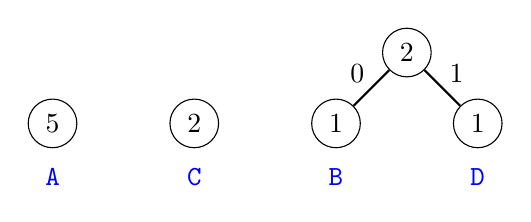
\begin{tikzpicture}[scale=0.9]
\node[draw, circle] (1) at (0,0) {$5$};
\node[draw, circle] (3) at (2,0) {$2$};
\node[draw, circle] (2) at (4,0) {$1$};
\node[draw, circle] (4) at (6,0) {$1$};
\node[draw, circle] (5) at (5,1) {$2$};

\node[color=blue] at (0,-0.75) {\texttt{A}};
\node[color=blue] at (2,-0.75) {\texttt{C}};
\node[color=blue] at (4,-0.75) {\texttt{B}};
\node[color=blue] at (6,-0.75) {\texttt{D}};

\node at (4.3,0.7) {0};
\node at (5.7,0.7) {1};
\path[draw,thick,-] (2) -- (5);
\path[draw,thick,-] (4) -- (5);
\end{tikzpicture}
\end{center}
Después de esto, los nodos con peso 2 se combinan:
\begin{center}
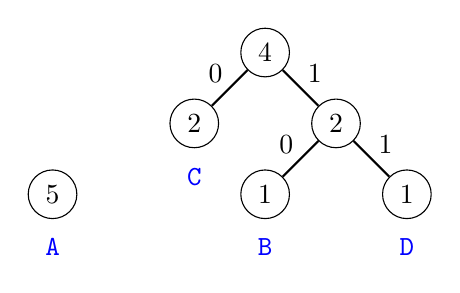
\begin{tikzpicture}[scale=0.9]
\node[draw, circle] (1) at (1,0) {$5$};
\node[draw, circle] (3) at (3,1) {$2$};
\node[draw, circle] (2) at (4,0) {$1$};
\node[draw, circle] (4) at (6,0) {$1$};
\node[draw, circle] (5) at (5,1) {$2$};
\node[draw, circle] (6) at (4,2) {$4$};

\node[color=blue] at (1,-0.75) {\texttt{A}};
\node[color=blue] at (3,1-0.75) {\texttt{C}};
\node[color=blue] at (4,-0.75) {\texttt{B}};
\node[color=blue] at (6,-0.75) {\texttt{D}};

\node at (4.3,0.7) {0};
\node at (5.7,0.7) {1};
\node at (3.3,1.7) {0};
\node at (4.7,1.7) {1};

\path[draw,thick,-] (2) -- (5);
\path[draw,thick,-] (4) -- (5);
\path[draw,thick,-] (3) -- (6);
\path[draw,thick,-] (5) -- (6);
\end{tikzpicture}
\end{center}
Finalmente, los dos nodos restantes se combinan:
\begin{center}
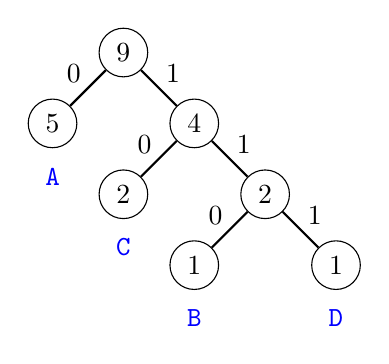
\begin{tikzpicture}[scale=0.9]
\node[draw, circle] (1) at (2,2) {$5$};
\node[draw, circle] (3) at (3,1) {$2$};
\node[draw, circle] (2) at (4,0) {$1$};
\node[draw, circle] (4) at (6,0) {$1$};
\node[draw, circle] (5) at (5,1) {$2$};
\node[draw, circle] (6) at (4,2) {$4$};
\node[draw, circle] (7) at (3,3) {$9$};

\node[color=blue] at (2,2-0.75) {\texttt{A}};
\node[color=blue] at (3,1-0.75) {\texttt{C}};
\node[color=blue] at (4,-0.75) {\texttt{B}};
\node[color=blue] at (6,-0.75) {\texttt{D}};

\node at (4.3,0.7) {0};
\node at (5.7,0.7) {1};
\node at (3.3,1.7) {0};
\node at (4.7,1.7) {1};
\node at (2.3,2.7) {0};
\node at (3.7,2.7) {1};

\path[draw,thick,-] (2) -- (5);
\path[draw,thick,-] (4) -- (5);
\path[draw,thick,-] (3) -- (6);
\path[draw,thick,-] (5) -- (6);
\path[draw,thick,-] (1) -- (7);
\path[draw,thick,-] (6) -- (7);
\end{tikzpicture}
\end{center}

Ahora todos los nodos están en el árbol, por lo que el código está listo.
Las siguientes palabras de código se pueden leer del árbol:
\begin{center}
\begin{tabular}{rr}
carácter & palabra de código \\
\hline
\texttt{A} & 0 \\
\texttt{B} & 110 \\
\texttt{C} & 10 \\
\texttt{D} & 111 \\
\end{tabular}
\end{center}
